\section{Motivation}



\section{Messverfahren}
Bei dem Messverfahren werden Öltröpfchen in einen Kondensator gesprüht. Daraufhin wird eine Spannung im Kondensator angelegt.
Durch ein Mikroskop lässt sich die Bewegung der Tröpchen beobachten. Jetzt wird gezielt ein Tröpfin mit langsamer Aufwärtsbewegung gewählt, da das Ziel ist eine einfach geladenes Tröpchen zu messen.
Von diesem mit einer Skala und aus- und einschalten die Steig- und Fallzeiten gemessen.
Daraus lässt sich dann die Elementarladung bestimmen.

\begin{figure}[h!]
    \centering
    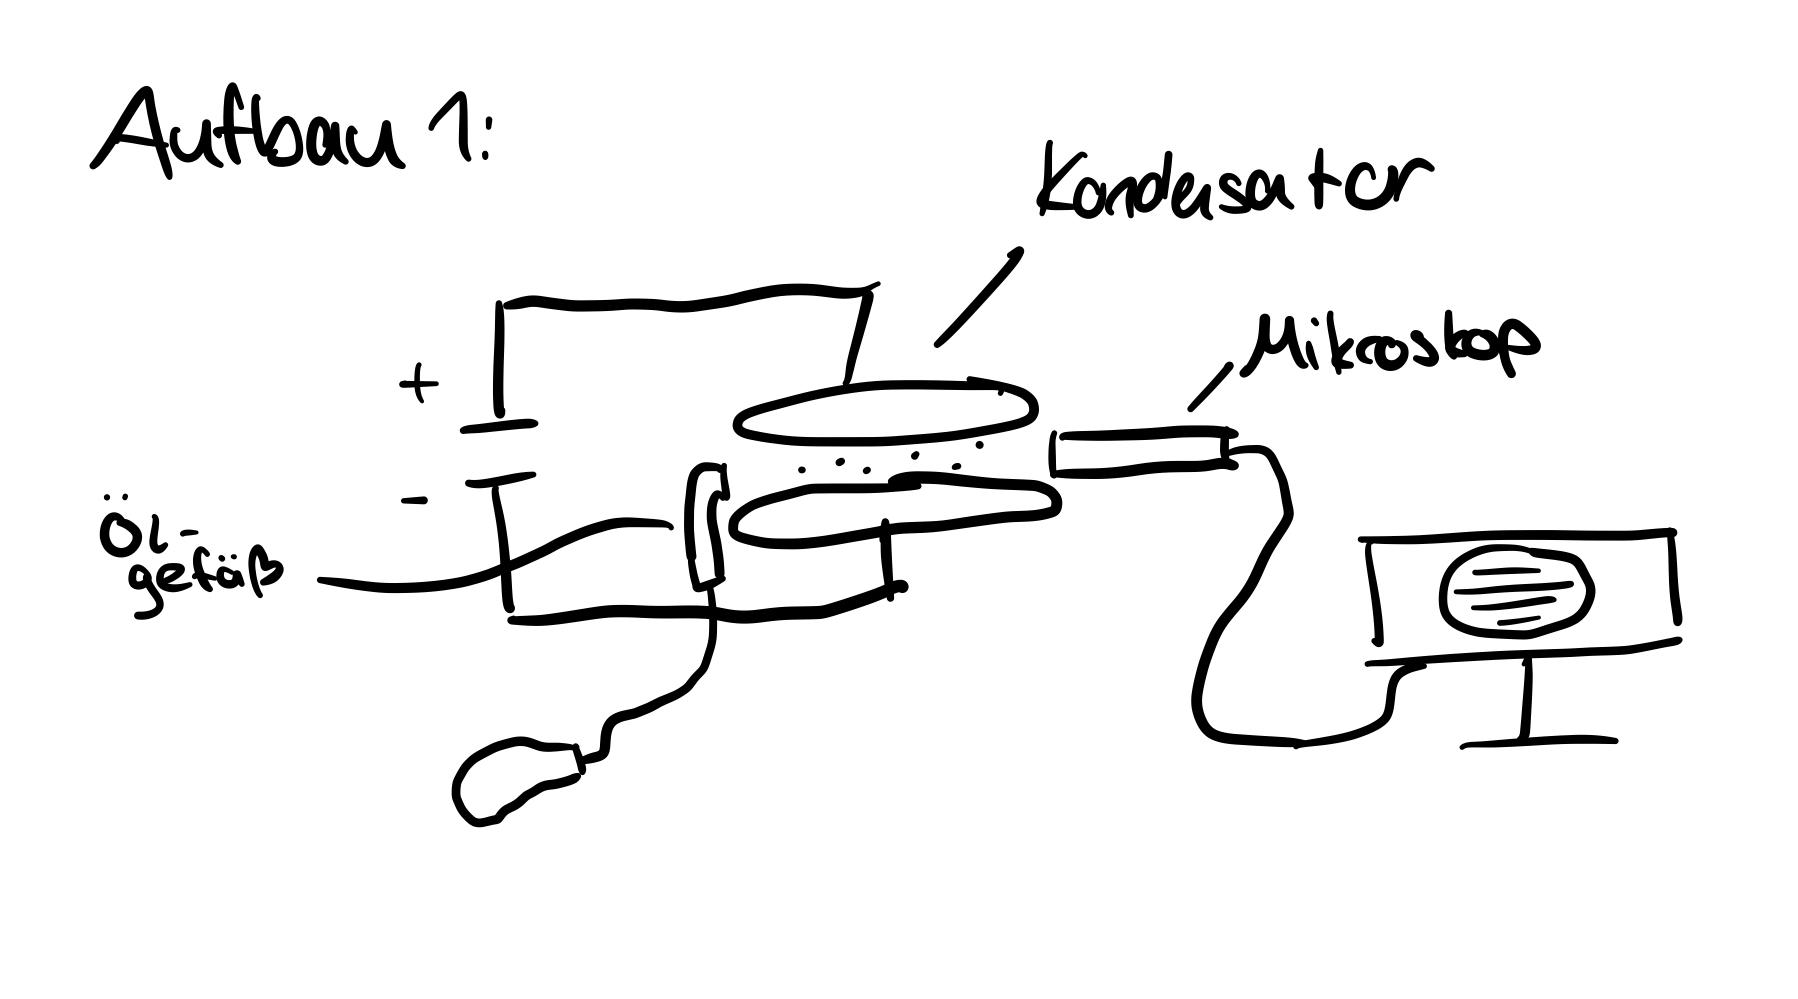
\includegraphics[width = .5\textwidth]{Aufbau.jpeg}
    \caption{Aufbau}
\end{figure}

\section{Grundlagen aus der Physik}
\subsection{Gravitationskraft}

Die Gravitationskraft einer Masse $m$ berechnet sich nach Newton durch:

\begin{equation}
    F_g = mg
\end{equation}
Wobei $g$ die Erdbeschleunigung ist. Setzt man nun $m=\frac{4}{3}\pi r^3 \rho$
Daras folgt für die Gravitationskraft:
\begin{equation}
    F_g = \frac{4}{3}\pi r^3 \rho g
\end{equation}s
Mit $r$ als Radius der Tröpfchen, näherungsweise eine Kugel. Und $\rho$ als Dichte des Tröpchens.
\subsection{Auftriebskraft}
Die Auftriebskraft entwpicht genau der Gewichtskraft der verdrängten Luft. Daraus folgt:
\begin{equation}
    F_A = \frac{4}{3}\pi r^3 \rho_{Luft} g
\end{equation}
Mit $\rho_{Luft}$ als Dichte der Luft und $r$ als Radius des Tröpfchen.

\subsection{Stokesche Reibung}
Bewegt sich eine Kugel durch ein Ideales Fluid erfährt sie eine Reibung in Abhängigkeit des Radius $r$, der dynamischen Viskosität $\eta$ und der Geschwindigkeit $v$.
Für die Reibung gilt folgende Gleichung, da Luft näherungsweise als ideales Gas betrachtet werden kann.
\begin{equation}
    F_R = 6 \pi r \eta v
\end{equation}

\subsection{Elektrische Kraft}
Da sich das Träpchen in einem elektrischen Feld bewegt, erfährt es eine Spannung durch die angelegte Spannung $U$.
In einem Plattenkondensator ergibt sich diese Kraft als:
\begin{equation}
    F_e = q\frac{U}{d}
\end{equation}
Wobei $d$ der Plattenabstand des Kondeensators ist.

\subsection{Kräftegleichgewicht}
Aus den Kräften ergibt sich für die Fallende bewegung:
\begin{equation}
    F_g = F_{R1} + F_A
\end{equation}
und beim steigen:
\begin{equation}
    F_G + F_{R2} = F_A + F_e
\end{equation}

Die Reibung wirkt immer entegegen der Bewegung, weshalb sie beim steigen auf die Gewichtskraft addiert wird.

Durch das einsetzen der Kräfte lässt sich die Gleichung für die Fallende Bewegung nach $r_0$ Auflösen, wobei $\eta_0$ die Viskosität ohne Korrekturfaktor ist.
\begin{equation}
    r_0 = \sqrt{\frac{9 \eta_0}{2 (\rho_{Öl}- \rho_{Luft}) g} v_f} \label{eq:r0}
\end{equation}

Setzt man nun die Gewichtskraft der fallenden Bewegung in die steigende ein erhält man:

\begin{equation}
    \Rightarrow F_e = F_{R2} + F_{R1}
\end{equation}

Setzt man hier erneut die Kräfte ein, lässt sich die Gleichung nach $q$ auflösen.

\begin{align}
    &q = (v_f + v_s)\sqrt{\frac{9 v_f\ (f\eta_0)^3}{2 (\rho_{Öl}- \rho_{Luft}) g}}\frac{6 \pi d}{U} \\ \label{eq:q}
\end{align}

\subsection{Korrektur der Viskosität}

Unterschreitet der Radius der Tröfchen die Weglänge der Luftmoleküle, kann die Abhängigkeit der Viskosität vom Radius nicht mehr al linear betrachtet werden.
Bei kleinen Wegängen entstehen nicht mehr ausreichen viele Kollisionen mit den Luftmolekülen, weshalb hier die Viskosität nach unten korrigiert werden muss.
Anschaulich betrachten können die Tröpfchen ohne Kollision zwischen zwei Luftmolekülen hndurch "rutschen".

\begin{equation}
    f(r) = \frac{1}{1+\tfrac{b}{rp}}
\end{equation}

Hierbei gibt $p$ den Luftdruck an, $r$ den Radius und $b$ eine Konstante für den Korrekturfaktor.